\documentclass[12pt,a4paper]{article}
\usepackage[utf8]{inputenc}
\usepackage{amsfonts}
\usepackage{amssymb}
\usepackage{amsmath}
\usepackage{graphicx}
\usepackage{float}

% sets margin
\usepackage[hmargin=3cm,vmargin=2.5cm]{geometry}

% creates landscape pages
\usepackage{pdflscape}
\usepackage{pdfpages}

%\renewcommand{\rmdefault}{phv} % Arial
\renewcommand{\sfdefault}{phv} % Arial

% defining settings for textpos
\usepackage[absolute]{textpos}
\setlength{\TPHorizModule}{\paperwidth}
\setlength{\TPVertModule}{\paperheight}

% headers / footers
\usepackage{fancyhdr}
\pagestyle{fancy}
\fancyhf{}
\rhead{Assignment 1A}
\lhead{CSG2341: Intelligent Systems}
\rfoot{\thepage}
\lfoot{Martin Ponce, ID: 10371381}
\renewcommand{\footrulewidth}{0.5pt}

% defining landscape headers / footers
\fancypagestyle{fancylscape}{
	\fancyhf{}
	\renewcommand{\footrulewidth}{0pt}
	\renewcommand{\headrulewidth}{0pt}
	% header
	\begin{textblock}{0.05}[-0.5,-2](0,0)
		{\rotatebox{90}{CSG2341: Intelligent Systems}}
	\end{textblock}
		\begin{textblock}{0.05}[-0.5,-1](0,0)
		{\rotatebox{90}{Assignment 1A}}
	\end{textblock}
	\begin{textblock}{0.05}[-1,-0.109](0,0)
		{\rotatebox{90}{\rule{24.2cm}{0.5pt}}}
	\end{textblock}
	% footer
	\begin{textblock}{0.05}[-19,-4.28](0,0)
		{\rotatebox{90}{Martin Ponce, ID: 10371381}}
	\end{textblock}
		\begin{textblock}{0.05}[-19,-12.8](0,0)
		{\rotatebox{90}{\thepage}}
	\end{textblock}
		\begin{textblock}{0.05}[-18.7,-0.109](0,0)
		{\rotatebox{90}{\rule{24.2cm}{0.5pt}}}
	\end{textblock}
}

% adjusts padding between caption and figure
\setlength{\belowcaptionskip}{10pt}

% adds links to references and colors them blue
\usepackage{hyperref}
\hypersetup{colorlinks=true,
			linkcolor=blue,
			citecolor=black,
			urlcolor=blue}

% apa style referencing
\usepackage[sectionbib, natbibapa]{apacite}
\usepackage{chbibref}

% underlining text
\usepackage[normalem]{ulem}

% \citetapos for possesive citations
\newcommand{\citetapos}[1]{\citeauthor{#1}{\textcolor{black}{'s}} \citeyearpar{#1}}

% add multiline comments \begin{comment} \end{comment}
\usepackage{verbatim}

% add minted package for code highlighting, number per section
\usepackage[section]{minted}

% add tcolorbox package to style code
\usepackage{tcolorbox}
\tcbuselibrary{minted,skins}

% javacode style config
\newtcblisting{javacode}{
  listing engine=minted,
  colback=bg,
  colframe=black!80,
  listing only,
  minted style=monokai,
  minted language=java,
  minted options={linenos=true,texcl=true,fontsize=\scriptsize},
  left=1mm,
}

% consolecode style config
\newtcblisting{consolecode}{
  listing engine=minted,
  colback=bg,
  colframe=black!80,
  listing only,
  minted style=vim,
  minted language=console,
  minted options={texcl=true,fontsize=\scriptsize},
  left=1mm,
}

% define bg color for code highlighting
\definecolor{bg}{rgb}{0.20,0.20,0.20}

% listings package
\usepackage{listings}
% change label to code
\renewcommand\listingscaption{Java code}

% modify enumerate sub list
\renewcommand{\labelenumii}{\theenumii}
\renewcommand{\theenumii}{\theenumi.\arabic{enumii}.}
\renewcommand{\theenumiii}{\theenumii\arabic{enumiii}}
\renewcommand{\theenumiv}{\theenumiii.\arabic{enumiv}}

% number each equation per section
\numberwithin{equation}{section}

% tikz graphics package
\usepackage{tikz}
\usetikzlibrary{arrows,positioning, calc}
\tikzstyle{vertex}=[draw,fill=black!15,circle,minimum size=18pt,inner sep=0pt]

% front matter
\title{Edith Cowan University\\CSG2341\\Intelligent Systems\\Assignment 1A}
\author{Martin Ponce\\Student 10371381\\\\Tutor: Philip Hingston}
\date{\today}

\begin{document}

% title page
\newpage
\null  % Empty line
\nointerlineskip  % No skip for prev line
\vfill
\let\snewpage \newpage
\let\newpage \relax
\maketitle
\thispagestyle{empty}
\let \newpage \snewpage
\vfill

% toc
\newpage
\tableofcontents
\thispagestyle{fancy}

\newpage
\section{Introduction}

Facebook is one of today's leading Social Networking Sites (SNS). The company reports that as of June 2014, their network serves 1.32 billion users per month \citep{Facebook2014}, while \citet{Hampton2011} identified that 92\% of SNS users in their dataset were Facebook users. As Facebook expanded registration to users outside educational and professional institutions in September 2006 \citep{Facebook2014}, males and females alike were quick to adopt the technology at a fast paced rate \citep{Mazman2011}. This adoption rate has triggered a multitude of scientific research ``from widely different fields of inquiry'', attempting to explain the phenomenon of Facebook \citep[p. 983]{Caers2013}. 

This literature review focuses on research which examine the demographic differences relating to SNS use, with particular attention to the role of gender. Men are generally regarded as earlier adopters of technology compared to women. This is evident in findings by \citet{Pitkow1994}, where 95\% of Internet users were men, while \citet[p. 896]{Kimbrough2013} declares that during the first half of the 1990's, the Internet ``was mostly regarded as a technological boy's toy''. A decade later, \citet{Fallows2005} asserts that there are just as many females as there are males online. Research by \citet{Fogel2009} provides supporting evidence that men are also earlier adopters of SNS, finding that more men had established SNS accounts before women. However, the trend has shifted, with recent reports indicating that women now represent the majority of SNS users compared to men \citep{Duggan2013, Hampton2011}.

As the Internet user gender gap disappears, it is more important than ever to understand the differences between genders and its effects relating to personal SNS use, so that current social network sites and social network sites of the future are able to service both men and women equally. This literature review will explore those differences as expressed in the body of current research literature, focusing on three main themes: The motivational differences between men and women in SNS use, the implications of gender in SNS self-presentation, and the differences in SNS privacy concerns between genders.
\section{Idea}

The main tactic for this controller is fly defensively in order to conserve energy and survive until there are a two enemies left. Turns for the most part will focus on the energy blast sensor, in order to dodge as many of them as possible. When there are only two enemy saucers left in the arena, turning will focus on the enemy saucer sensor, to track them down and shoot at them from a close distance.

However, when any power ups spawn nearby, the goal is to move straight to the power up, ignoring any energy blasts. If any close energy blasts close to the player while attempting to retrieve a power up, the player will deploy the shield. The rate of fire will be kept to a minimum for most situations to conserve energy, unless a nearby power up spawns, or if there is only two remaining enemy saucers left. In these cases, the rate of fire will increase, to either deter enemy saucers from retrieving the power up, or attempt to destroy them.

Speed will also be kept at the minimum for most situations, only increasing speed when necessary for dodging, or when a power up spawns nearby, to try and get to it first. Speed will also be increased when there are only two remaining enemy saucers left, attempting to destroy them before the timer runs out.

This controller attempts to implement these strategies with turning, speed, shield deployment and firepower, with the primary goal of flying defensively by dodging energy blasts and retrieving nearby power ups. When there are only two enemies left, the saucer will begin to fly offensively, increasing speed and firepower, and attempt to destroy the enemies before the timer runs out.
\\
\\
The following strategy will be implemented:

\begin{itemize}
\item Fly defensively
	\begin{itemize}
	\item Try to stay away from the ``furball'', let the other saucers destroy each other
	\item Conserve energy
	\item Keep rate of fire to a minimum
	\item Focus movement on dodging energy blasts
	\end{itemize}
\item If a powerup spawns nearby
	\begin{itemize}
	\item Stop dodging energy blasts
	\item Move straight to the powerup at high speed
	\item If there are no close, incoming energy blasts, fire at maximum rate of fire to deter others from reaching the powerup
	\item If there are close, incoming energy blasts, deploy shield
	\end{itemize}
\item If there are only two enemies left
	\begin{itemize}
	\item React to any powerup, even those that are far, to starve the remaining enemies of extra power
	\item Fly aggressively
	\item Increase rate of fire
	\item Attempt to destroy remaining enemies before timer runs out
	\end{itemize}
\end{itemize}
\section{Input fuzzy variables}

\subsection{myEnergy}

The fuzzy variable \emph{myEnergy} is the player's energy level and determines whether or not the player has \emph{lowEnergy} or \emph{highEnergy} remaining. The universe of disclosure for \emph{myEnergy} is between 0 joules and 10,000 joules, the amount of energy that all saucers begin with.



\section{Output fuzzy variables}


\newpage

\section{Sample fuzzy rule}

\subsection{Turning rule}

This section will examine the implementation of the fuzzy rules that govern the saucer's ability to turn, and will use the following situation, as shown in Figure 4 to demonstrate how the \emph{turn} output rules are fired:

\begin{figure}[H]
\centering
\caption{Sample game screen}
\includegraphics[scale=1]{./img/png/gameScreen.png}
\end{figure}

The yellow saucer in Figure 4 is the \emph{player}, called \emph{checkSix}, while the enemy is the grey saucer, called \emph{fuzzy}. Note that \emph{fuzzy} is controlled with the original, existing fuzzy controller supplied with the assignment. Two \emph{turn} rules are fired during this sequence:

\begin{itemize}
	\item Rule 1:
		\begin{itemize}
			\item IF (\emph{heading angle} IS front) AND (\emph{energy difference} IS winning) THEN (\emph{turn} IS 0)
		\end{itemize}	 
	\item Rule 2:
		\begin{itemize}
			\item IF (\emph{heading angle} IS left front) AND (\emph{energy difference} IS winning) THEN (\emph{turn} IS 90)
		\end{itemize}
\end{itemize}

\subsubsection{\emph{Energy difference} antecedent}

\emph{Energy difference} will be explored first, since the value is the same in both instances of Rule 1 and Rule 2 above. The \emph{energy difference} antecedent, which in this case is \emph{winning}, is demonstrated by the difference of energy between the two saucers. \emph{checkSix} has 3940.71 joules of energy remaining, while \emph{fuzzy} only has 264.74. The \emph{energy difference} is +3675.97j. Therefore, \emph{checkSix} is \emph{winning}. Figure 5 below demonstrates the firing of this antecedent, and shows that the fuzzy set value is +3675.97, while $\mu$, the membership value to the \emph{winning} fuzzy set, is 1.

\begin{figure}[H]
\centering
\caption{\emph{Energy difference} antecedent}
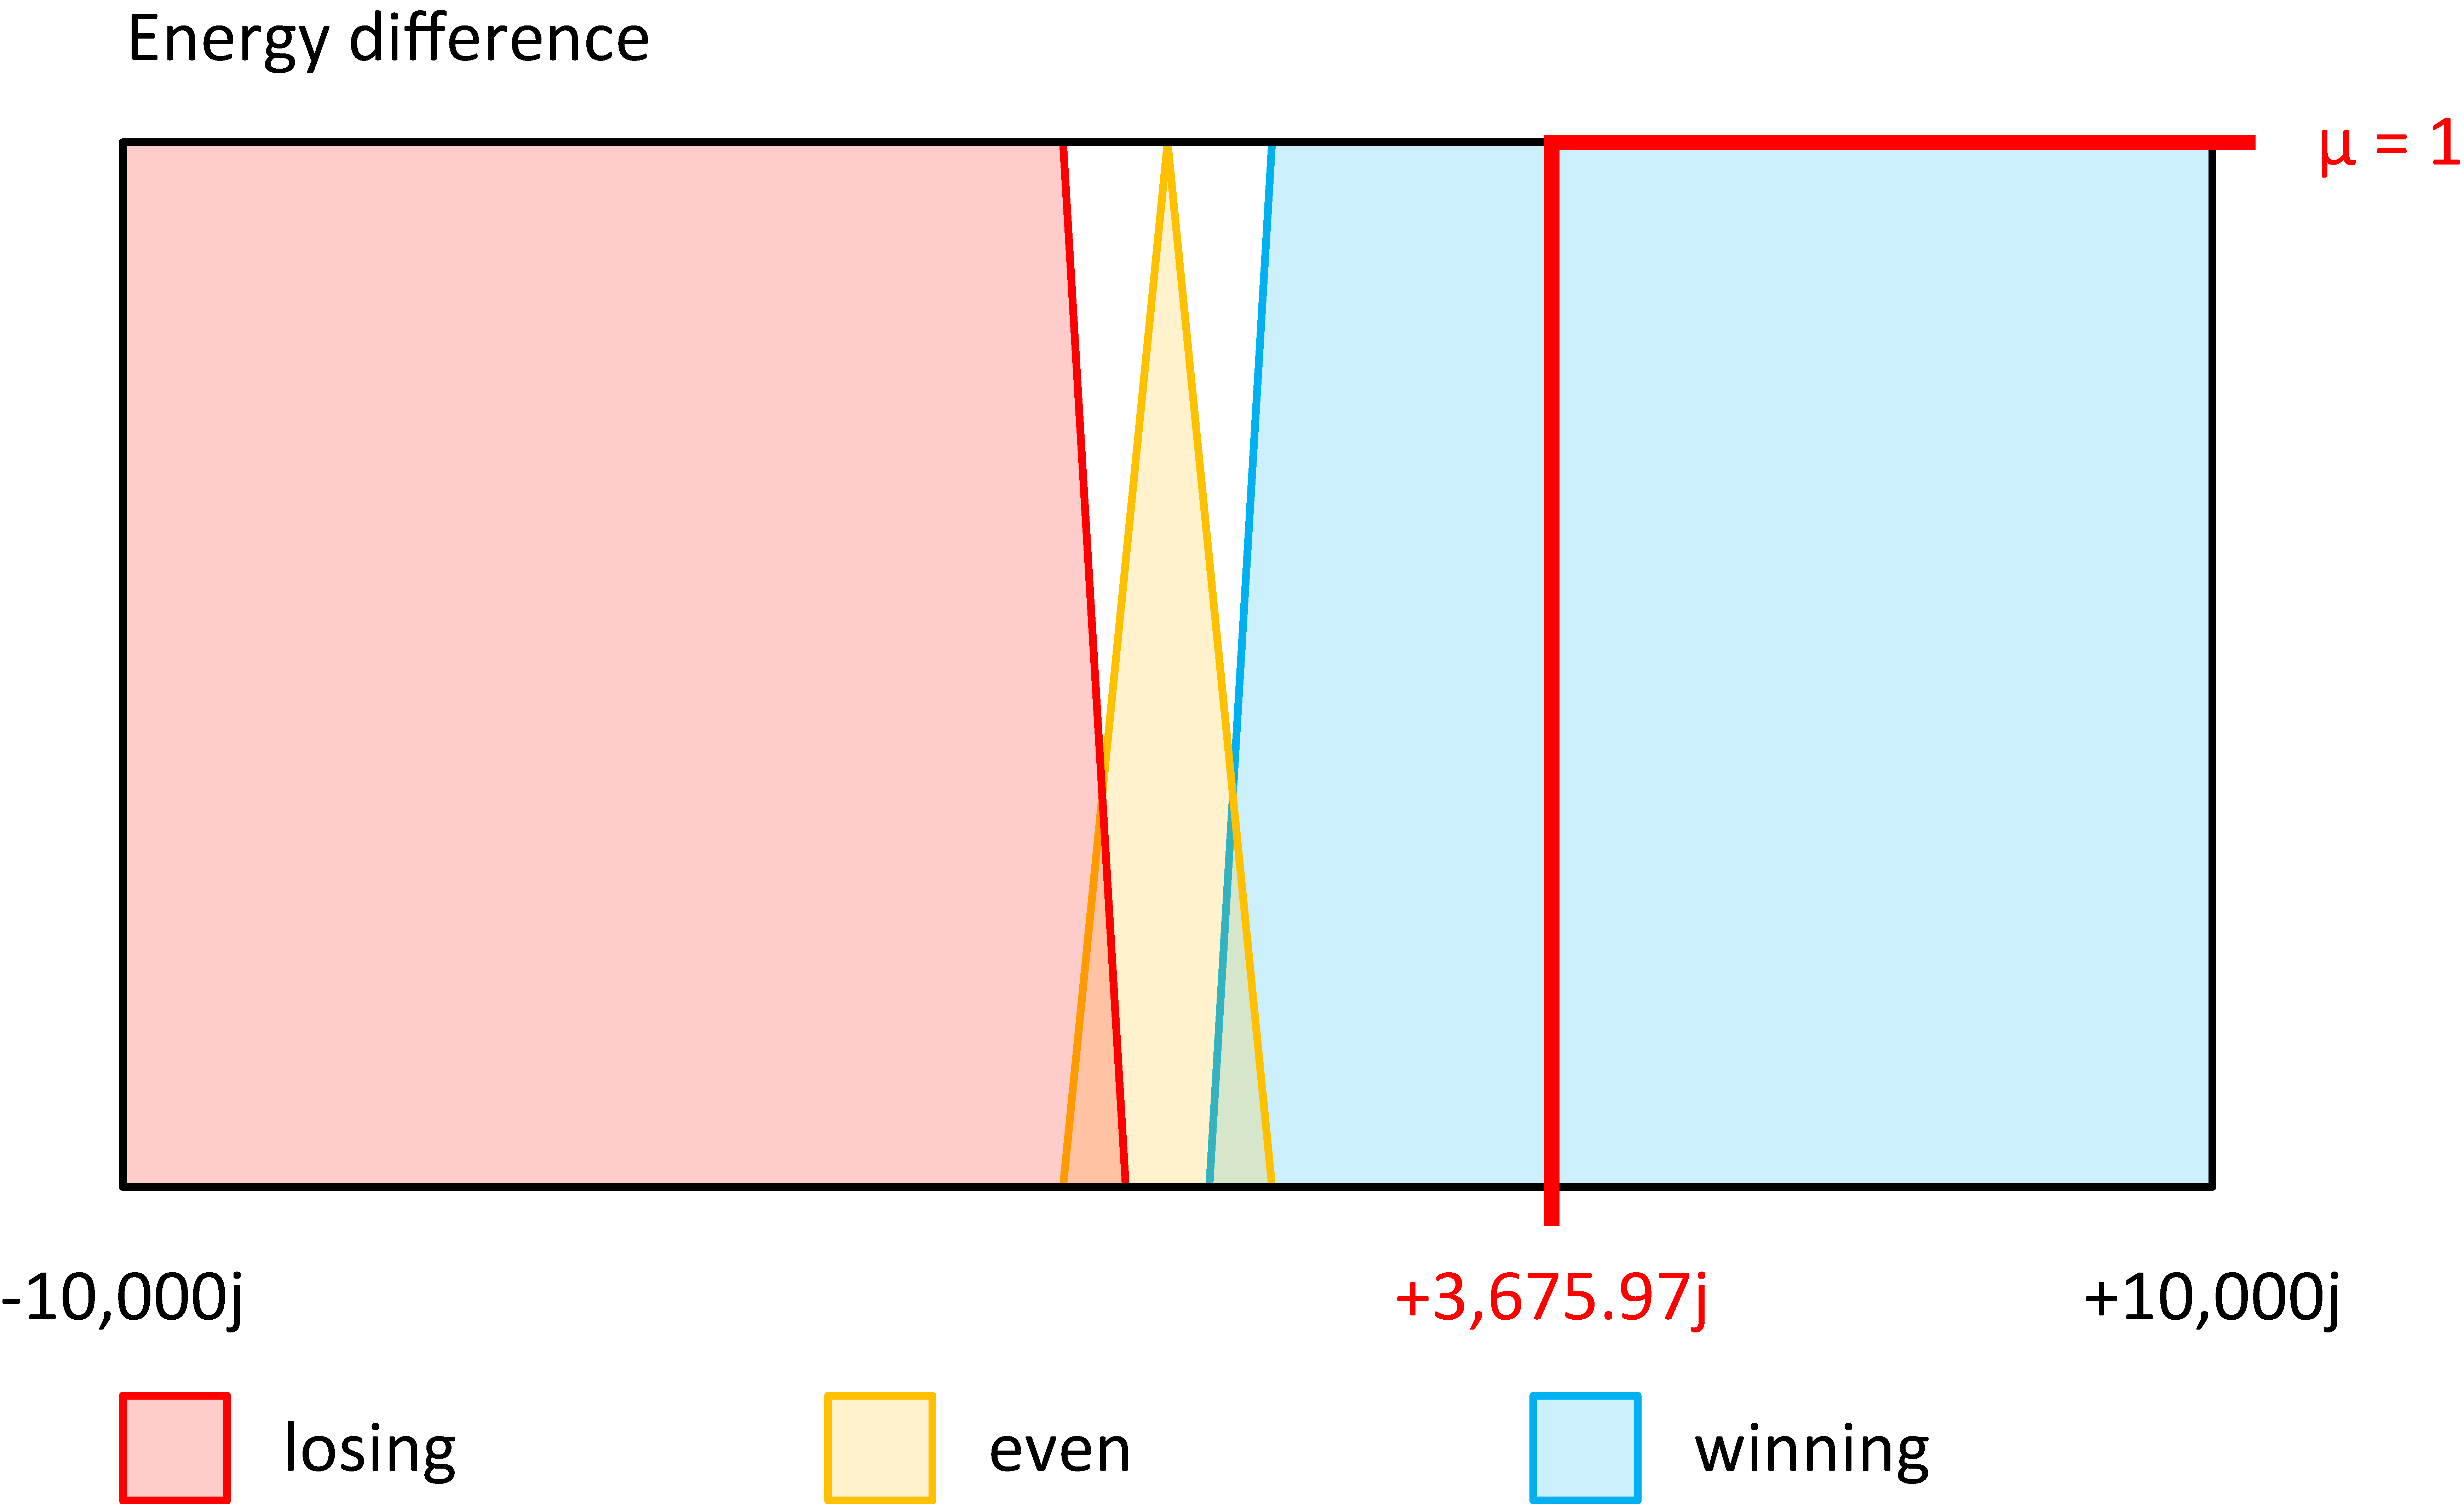
\includegraphics[scale=0.1]{./img/pdf/turnRule_energyDiff.pdf}
\end{figure}

\subsubsection{\emph{Heading angle} antecedent}

\emph{Heading angle} causes Rule 1 and Rule 2 to fire, with \emph{front} and \emph{leftFront}. This is due to the configuration of the two fuzzy sets. As seen previously in Figure 3, the \emph{leftFront} fuzzy set begins at 50\% of the \emph{front} fuzzy set range. In other words, any value higher than the median value of \emph{front} will also belong to the \emph{leftFront} set. Conversely, any value lower than the median value of \emph{front} will also belong to the \emph{rightFront} set. Figure 6 below demonstrates the firing of these two antecedents, their fuzzy set values and their $\mu$ values.

\begin{figure}[H]
\centering
\caption{\emph{Heading angle} antecedent}
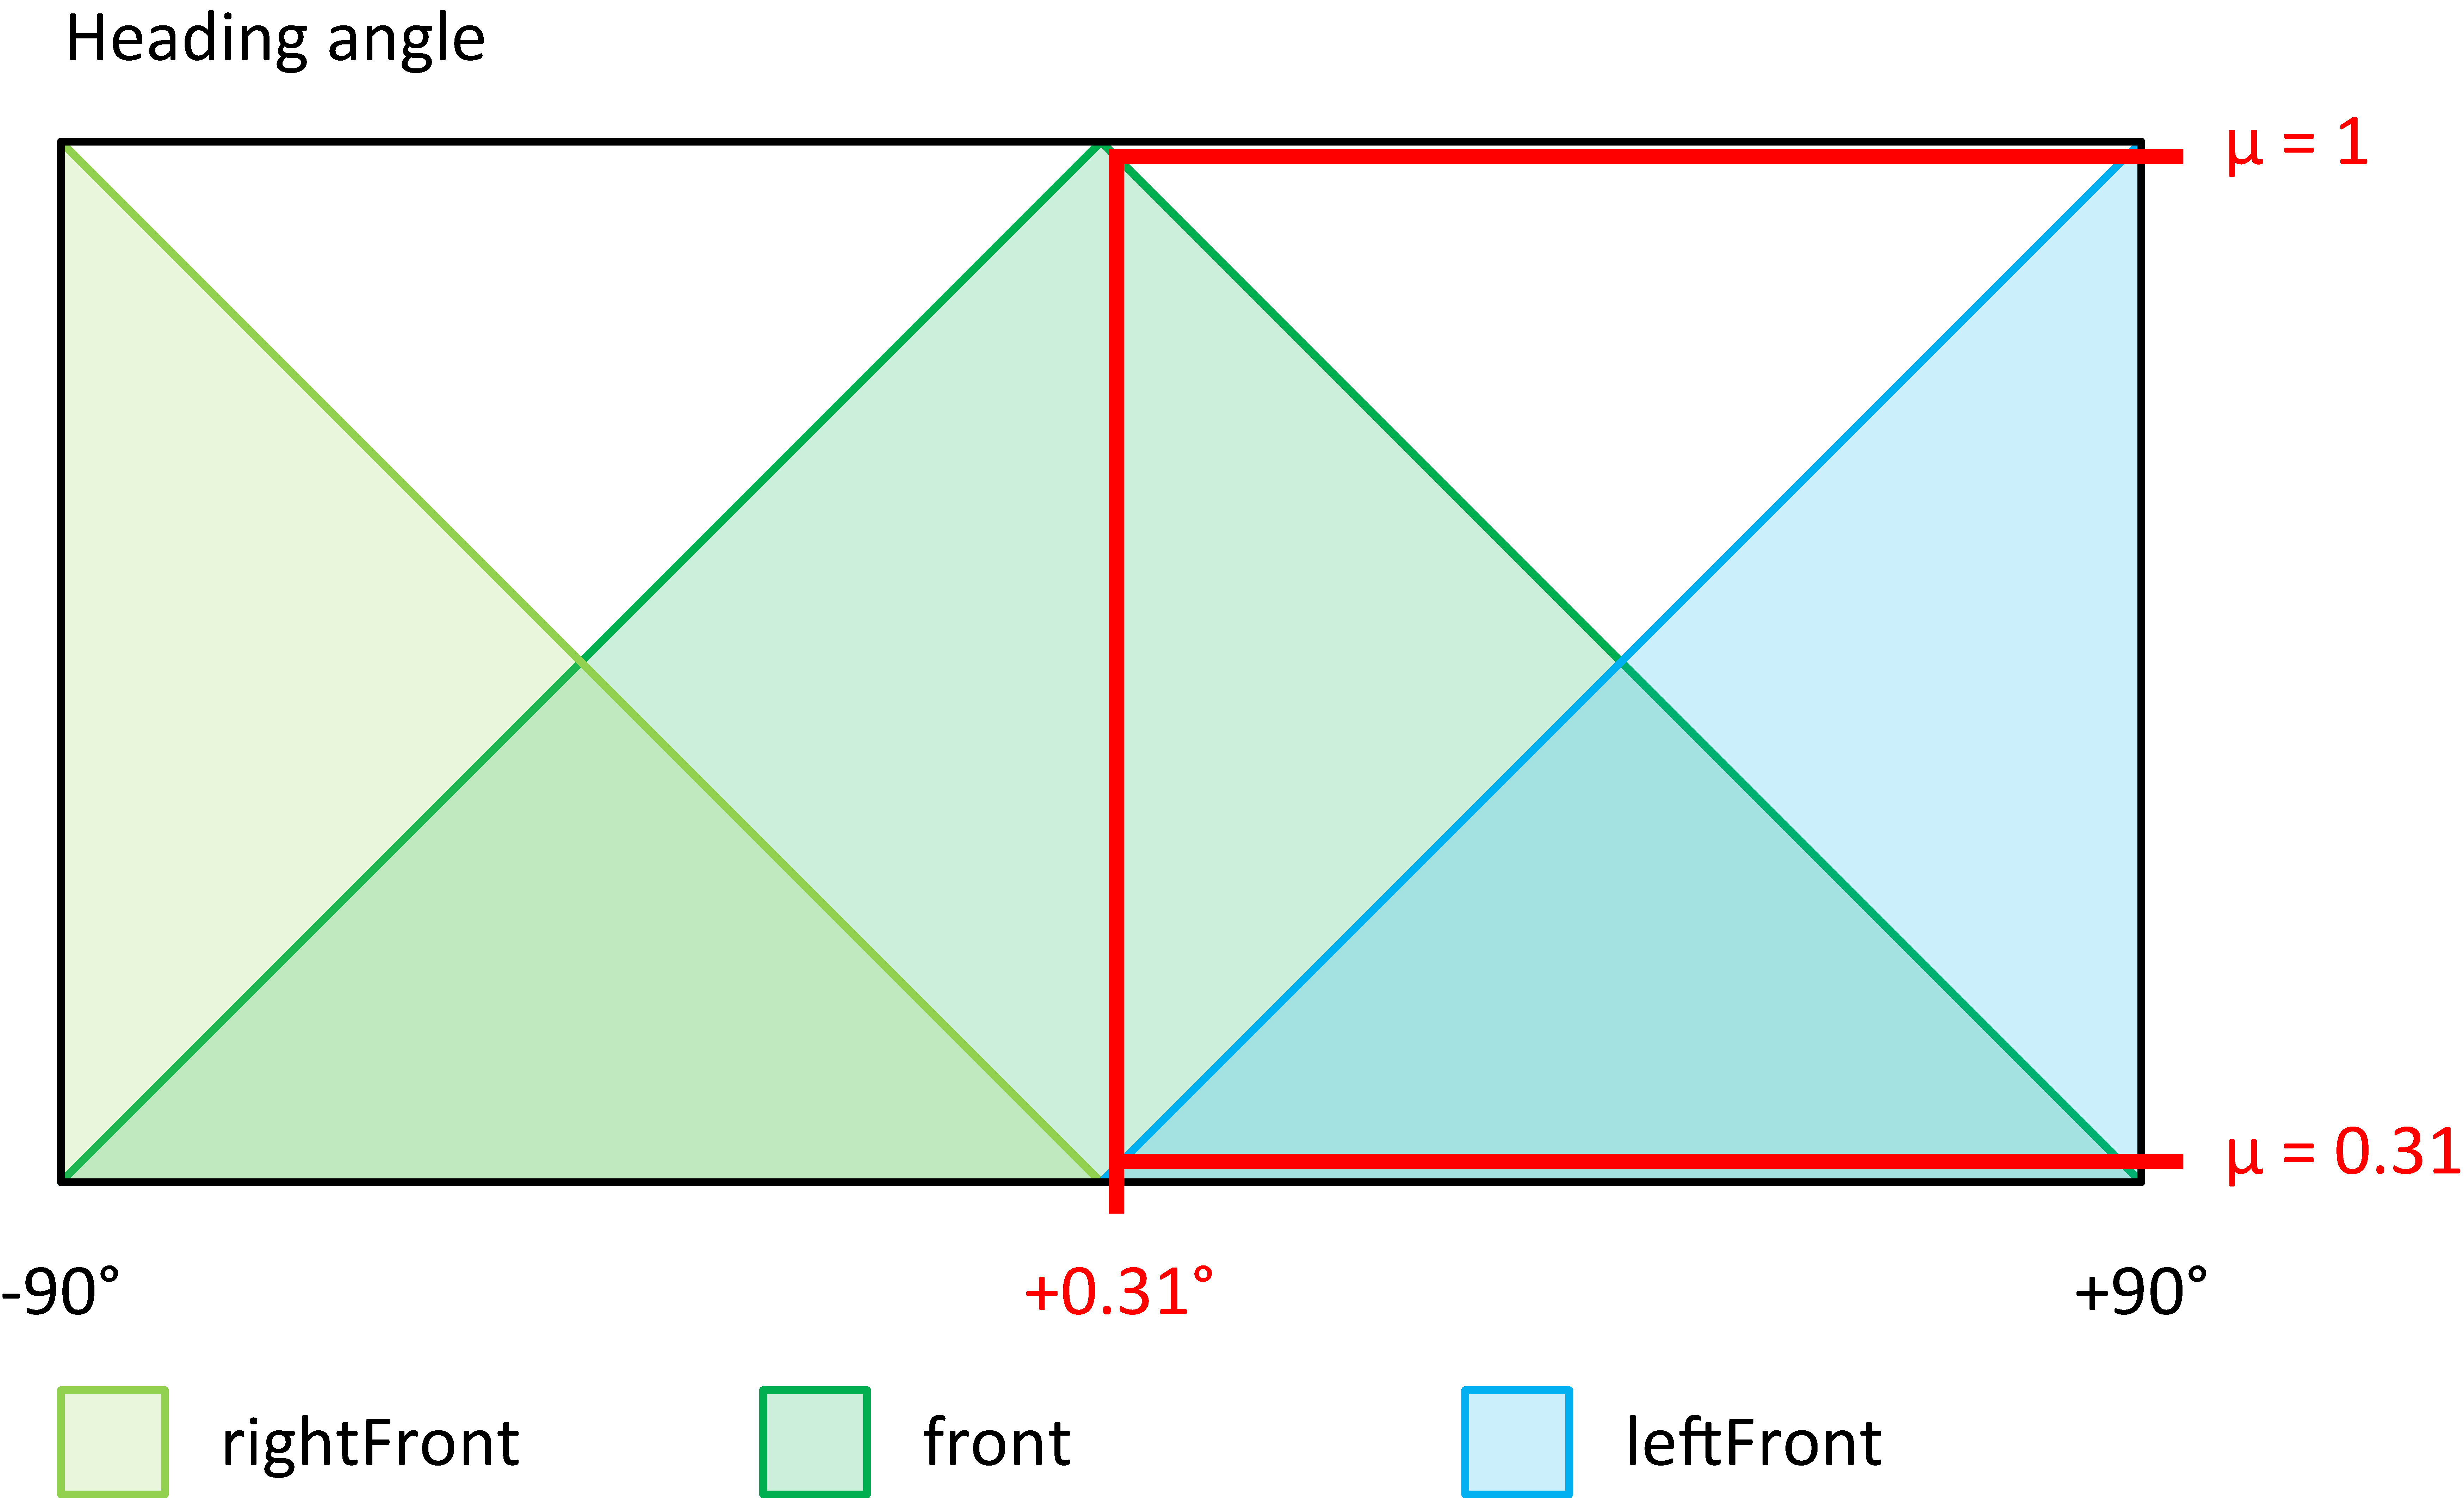
\includegraphics[scale=0.1]{./img/pdf/turnRule_headingAngle.pdf}
\end{figure}

Figure 6 shows a simplified view of the \emph{heading angle} sets, only displaying -90$^{\circ}$ to +90$^{\circ}$ during the firing of Rule 1 and Rule 2. The \emph{heading angle} value of +0.31$^{\circ}$ belongs to the \emph{front} fuzzy set at $\mu$ = 1, and also belongs to the \emph{leftFront} fuzzy set at $\mu$ = 0.31, hence the firing of the two rules, thus providing two inputs. These inputs, along with the \emph{energy difference} input will be aggregated to create a single, crisp output, as explained in the next section.

\subsubsection{Rule aggregation}

When multiple inputs are provided by the same linguistic variable antecedent, as seen in Section 4.1.2, Sugeno style inference calculates the weighted average to provide a single, crisp input, using the following formula:

{\LARGE
	\begin{align}
	\mbox{WA} = \frac{\sum^N_{i=1} \mu(k_i) k_i}{\sum^N_{i=1} k_i}
	\end{align}
}

\noindent
Therefore, to calculate the weighted average for the two \emph{heading angle} inputs for the example shown in Figure 6:

{\LARGE
	\begin{align}
	\mbox{WA} &= \frac{1 \times 0.31 + 0.31 \times 0.31}{1 + 0.31} \\
	&= 0.31
	\end{align}
}

\noindent
Subsequently, the crisp output from the two \emph{heading angle} antecedents is 0.31. However, $\mu$ for the \emph{energy difference} antecedent must also be considered. As discussed in Section 4.1.1, $\mu$ = 1 for \emph{energy difference}.

Since the example rule performs an AND operation between the two antecedents, fuzzy set operations dictate that an intersection operation must occur to determine the final, crisp output. Therefore, the following function is appropriate:

{\LARGE
	\begin{align}
	\mbox{output} = \mbox{min}(\mu(k_1), \mu(k_2), \mbox{...}, \mu(k_n))
	\end{align}
}

\noindent
When applied to our example rules that have been fired:

{\LARGE
	\begin{align}
	\mbox{output} &= \mbox{min}(1, 0.31) \\
	&= 0.31
	\end{align}
}

\noindent
Therefore, the final, crisp output for the example scenario is a turn of 0.31$^{\circ}$. In other words, from its current direction of 0.0$^{\circ}$, the saucer will turn LEFT for 0.31$^{\circ}$, in order to follow the enemy, who is in front, and slightly to the left.
\newpage

\section{Learnings}

Although I believe I have a firm grasp on the basic concepts of fuzzy logic, I had a considerable amount of trouble understanding the logic behind \emph{turning} the saucer. I ran several tests, printing the opponent direction values during runtime to understand the relationship between where the player saucer is, and where the enemy is, and the values that were returned each frame. It was only until I imagined that the negative, right-hand turn values as ``turning counter-clockwise'' did I manage to tune the turn rules to a working manner.

My initial concept was to aggressively attack the opponent as soon as the game started, which worked fine. However, I could not test my defensive strategy, and initially just hoped that my saucer would immediately overcome the enemy with firepower and always be within the ``winning'' fuzzy set limits. Eventually, I realised that the original \mintinline{console}{FuzzyController.java} class could be made more difficult by changing the values, as listed below:

\begin{listing}[H]
\caption{FuzzyController.java modifications}

\begin{javacode}
public FuzzyController() throws Fuzzy Exception {
  // ...
  final double maxPower = Saucer.MAX_POWER;
  final double midPower = maxPower; // originally divided by 5.0
  final double lowPower = maxPower; // originall divided by 20.0
  // ...
}
\end{javacode}
\end{listing}

In doing so, the opponent always fires at maximum power when close, testing whether or not my offensive strategy to always stay right next to the enemy worked. Initial tests proved that my strategy did not work and was destroyed immediately. I needed to develop a substantial defensive strategy.

The heading angle fuzzy sets were modified from my original, arbitrarily chosen sets, to sets that are based on clock positions in relation to the player's position, similar to what a fighter pilot might say during combat, ie. ``Bandit at my six o'clock'', or ``Bogey at my nine''. The turn output spikes were also chosen based on the clock analogy, resulting in much more controlled behaviour, and enabled me to define a defensive strategy through the turn rules.

However, the rules require refinement, as confusion can occur when the player saucer hits a battle space border and the opponent direction being returned switches between negative and positive values. This confusion results in the player saucer spinning on the spot, and would be a major problem if turns cost energy. Firepower could also be improved by refining input sets or rules. Currently, the player saucer may fire weak shots even though the enemy is far away, resulting in wasted energy.

My offensive strategy is also far from perfect and has much room for improvement. Sitting right behind the enemy and giving chase during offence may suit well to space/aircraft with fixed, forward facing armament, but is a dangerous place to be when the enemy can rotate his weapon to face the rear.
\section{Conclusion}

The aim of this research paper is to explore the relationships between gender and Facebook use. Observations were collected from 48 fictional participants from a survey and the following thesis statements were tested by comparing gender and the number of Facebook friends, the number of close friends, the Sociability score and reported Facebook hours. 

Out of the total 48 participants, only 3 were women. The data collected from the participants were identified as non-normally distributed, and therefore non-parametric tests were selected. 

\subsection{Thesis statement 1: Gender is related to the size of a user's Facebook network}

This research paper's literature review discovered that there were conflicting views on the topic of gender and network size. Gender was compared with Facebook friends to find any supporting evidence that gender is related to the size of a user's Facebook network.

Spearman's correlation coefficient test and Wilcox rank sum test both indicate that there is no correlation between gender and Facebook friends, however due to the small number of female participation, no conclusions can be made with the results.

Secondary variables were also explored, testing Close friends and Sociability with gender, which may have provided further evidence towards the thesis statement. Both non-parametric tests indicate that there is no correlation between gender and Close friends or Sociability. With such a small number of female participants, no conclusions can be made with the results.

\subsection{Thesis statement 2: Gender is related to the amount of time a user spends on Facebook}

The literature review suggested that women are attracted to the social aspect of Facebook and SNS more than men. This research paper aimed to explore that statement by comparing gender with reported Facebook hours.

Again, both non-parametric tests found that there is no correlation between gender and Facebook hours. However, there is not enough evidence from female participants for conclusions to be made with the results.

\subsection{Limitations}

Due to the small amount of female representation in the sample set, no conclusions from the test results could be made, and posed a recurring limitation in this research paper. Further research is recommended with a sample set that includes an equal balance between male and female participants. Actual Facebook friend numbers rather than self-reported estimates would also further enhance any future study results.

\newpage
\urlstyle{rm}
\bibliographystyle{apacite}
\addcontentsline{toc}{section}{References}
\bibliography{./bib/Year_2-Sem_1-CSG2341-0b_A1}


\end{document}